\documentclass[a4paper, 10pt, twocolumn, preprint, 3p]{elsarticle}

%% AMS packages provides various useful mathematical features
\usepackage{amsfonts, amsmath, amssymb, amsthm}
%% Other mathematical packages: arrays, vectors, IEEE equations and mathtools 
\usepackage{array, booktabs, multirow}
\usepackage{esvect}	
\usepackage[retainorgcmds]{IEEEtrantools}
\usepackage{mathtools}
%% Fonts
\usepackage{bbm, dsfont, mathrsfs}		
\usepackage[T1]{fontenc}
%% Footnotes
\usepackage{footmisc}
\usepackage{fnpct}
%% Landscape tables
\usepackage[figuresright]{rotating}
%% URL references
\usepackage[hyphens]{url}
%% Line numbers
\usepackage{lineno}
	\modulolinenumbers[5]
%% Hypertext references
\usepackage{hyperref}

%%=========================================================================================%%
\newcommand{\sqrts}[2][]{\,\sqrt[#1]{#2}\,}

\def\E{\mathbb{E}}
\def\el{l}
\def\given{\,|\,}
\def\I{\mathbb{I}}
\def\N{\mathbb{N}}
\def\one{\mathds{1}}
\def\P{\mathbb{P}}
\def\R{\mathbb{R}}
\def\S{\mathbb{S}}

\def\mwmwh{\delta}
\def\eff{\eta}

%%=========================================================================================%%
\journal{Renewable Energy}

%%=========================================================================================%%
%% Hyphenation exception list
\hyphenation{}

%%=========================================================================================%%
%% Elsevier bibliography styles

%% Numbered
%\bibliographystyle{model1-num-names}
%% Numbered without titles
%\bibliographystyle{model1a-num-names}
%% Harvard
%\bibliographystyle{model2-names.bst}\biboptions{authoryear}
%% Vancouver numbered
%\usepackage{numcompress}\bibliographystyle{model3-num-names}
%% Vancouver name/year
%\usepackage{numcompress}\bibliographystyle{model4-names}\biboptions{authoryear}
%% APA style
%\bibliographystyle{model5-names}\biboptions{authoryear}
%% AMA style
%\usepackage{numcompress}\bibliographystyle{model6-num-names}
%% `Elsevier LaTeX' style
\bibliographystyle{elsarticle-num}

\begin{document}
%%=========================================================================================%%
%% FRONT MATTER																			%%
%%=========================================================================================%%
\begin{frontmatter}

\title{Firming wind power dispatch with battery energy storage}

\author[acems]{Primary Author\corref{corauthor}}
\cortext[corauthor]{Corresponding author.}
\ead{primary.author@adelaide.edu.au}

\author[acems]{Co-Authors}

\address[acems]{School of Mathematical Sciences and\\ARC Centre of Excellence for Mathematical \& Statistical Frontiers,\\The University of Adelaide, South Australia, 5005}

\begin{abstract}
Battery energy storage provides a means of firming the dispatch of power generated from variable renewable energy sources including wind.  We conjecture that firming wind power dispatch with battery energy storage would dampen the volatility of wholesale electricity prices, leading to lower prices.  In order to measure the effect of battery energy storage on firming wind power dispatch, we develop a multi-period incremental state-space model that improves on prior models in the literature by properly accounting for charge/discharge efficiency and penalising control effort.  We apply model predictive control with mixed integer quadratic programming to minimise the tracking error of power (wind and battery) dispatched to the grid relative to power schedule during pre-dispatch on the basis of unconstrained intermittent generation forecasts.  Conducting virtual trials over a one-year simulation horizon, we conclude that much of the wind forecast error can be offset by power supplied to, or discharge from, a relatively small battery.
\end{abstract}

\begin{keyword}
Wind power dispatch \sep battery energy storage \sep incremental state-space model \sep model predictive control \sep mixed integer quadratic programming \sep unconstrained intermittent generation forecasts \sep virtual trials
%\MSC[2010] 00-01\sep  99-00
\end{keyword}

\end{frontmatter}

%\linenumbers		% Activate line numbers
%%=========================================================================================%%
%% INTRODUCTION																			%%
%%=========================================================================================%%
\section{Introduction}\label{sect:introduction}
The Australian Energy Market Operator (AEMO) reports that in fiscal year 2016--17, 48.4\% of the electricity generated in the state of South Australia came from intermittent renewable energy sources --- 39.2\% wind and 9.2\% rooftop photovoltaic --- and 50.5\% from natural gas \cite{SAER17}.  During the month of July 2016 the wholesale electricity price averaged AUD 229/MWh in SA, more than three times the average price for any other region of the national electricity market (NEM).  In drawing lessons from the events of July 2016, \cite{WB16} attributed the soaring wholesale electricity price in SA to a combination of high penetration of intermittent renewable energy generation, limited connectivity with other regions in the NEM and historically high wholesale gas prices.  At the trading interval level, the Australian Energy Regulator (AER) publishes a report identifying significant contributing factors whenever the wholesale electricity price exceeds AUD 5,000/MWh.  With electricity trading at AUD 7,068/MWh in SA on 13 July 2016, AER identified wind forecast error as the major contributing factor to the price spike \cite{AER16}: ``Semi-scheduled wind for the 6:30 am trading interval was forecast to be around 900 MW both four and 12 hours ahead and around 820 MW half an hour ahead.  Actual semi-scheduled wind output was around 600 MW.''

We conjecture that if wind farms were to dependably supply power scheduled during pre-dispatch, then wholesale electricity prices would be less volatile and, on average, lower.  This paper applies state-space model predictive control (MPC) to firm the dispatch of wind power scheduled during pre-dispatch using battery energy storage to enable time shifting.

The contribution of this research is both theoretical and empirical.  Our theoretical contribution extends the single period, incremental state-space model of \cite{TREB16} to a multi-period setting.  The multi-period state-space model properly accounts for battery charge/discharge efficiency, and its incremental formulation allows the MPC controller to penalise control effort.  On an empirical level, we demonstrate the firming of wind power dispatch by simulating power dispatched to the grid by an SA wind farm coupled with a utility-scale battery.  Power is scheduled during pre-dispatch on the basis of unconstrained intermittent generation forecasts (UIGF) produced by the Australian Wind Energy Forecasting System (AWEFS).  We find that by minimising the tracking error of power (wind and battery) dispatched to the grid relative to scheduled power, much of the wind forecast error can be offset by power supplied to, or discharged from, a relatively small battery.

%A number of recent studies use state-space MPC to demonstrate the improvement in wind power dispatch with battery energy storage.  Their common objective is to minimise the tracking error of actual power dispatched to the grid relative to set points generated using, among other data, wind power forecasts.  They implemented MPC controllers that enabled wind farms to: schedule power dispatched to the grid \cite{HALBB14,TBBH10}; minimise cost by prolonging battery life \cite{KS10,YCTL12}; maximise revenue by exploiting energy arbitrage \cite{KKSA13}; or supply quality power through the provision of ancillary services \cite{YCTL14}.  Other than \cite{TREB16}, state-space models developed in prior papers are not of the incremental type, and do not penalise control effort.  Nor do they properly account for battery charge/discharge efficiency, instead, either assuming 100\% efficiency or approximating energy losses independent of the power stored or discharged during the dispatch interval.

We begin by reviewing prior papers that apply state-space MPC to demonstrate the improvement in the dispatchability of wind power using battery energy storage.  Section~\ref{sect:ssmpc_dispatch} provides a general overview of incremental state-space MPC, and proceeds to develop a multi-period model for wind power dispatch with battery energy storage.  In Section~\ref{sect:sa_wind_bess} we outline technical specifications of an SA wind farm and utility-scale batteries coupled to it, as well as parameters of the MPC controller.  Results from computer simulations of the MPC controller firming wind power dispatch with battery energy storage are reported in Section~\ref{sect:sim_wind_dptch_bess}.  We conclude this paper by proposing directions for future research.

%%=========================================================================================%%
%% LITERATURE REVIEW																		%%
%%=========================================================================================%%
\section{Literature Review}\label{sect:lit_review}
The single period state-space model of \cite{TREB16} properly accounts for battery charge/discharge efficiency, and its incremental formulation allows the MPC controller to penalise control effort.  The authors used state-space MPC to simulate power dispatched to the electricity grid by a wind farm coupled with a utility-scale, lithium-ion battery.  Implementing a na\"ive, single period dispatch strategy, they measured the improvement, at varying levels of confidence, in supplying a target baseload power that is calibrated to the daily load profile of the season, summer or winter.  Their empirical study finds that the probability of supplying the target baseload power is moderately higher with battery energy storage than no energy storage.  But, even on today's utility scale, battery power can only substitute for a fraction of the nameplate generation capacity of a commercial wind farm for a limited time.

Other than \cite{TREB16}, state-space models developed in prior papers are not of the incremental type, and do not penalise control effort.  Nor do they properly account for battery charge/discharge efficiency, instead, either assuming 100\% efficiency or approximating energy losses independent of the power stored or discharged during the dispatch interval.  The authors of \cite{HALBB14} used state-space MPC to demonstrate the improvement in wind power dispatch with battery energy storage in the US Pacific Northwest.  Their state-space model accounts for battery charge/discharge efficiency by including a power loss variable that depends on the power rating of the battery, but is independent of the power stored or discharged during the dispatch interval.  The primary objective of \cite{HALBB14} was to minimise the tracking error of actual power dispatched relative to scheduled power over a range of scheduling intervals.  The penalty applied to tracking error in the MPC performance index is reflective of the rate charged to wind generators for reserves used to balance the difference between scheduled and actual power generation.  Their state-space model is not an incremental one, so the authors left penalising control effort in the performance index for future research.  Unsurprisingly, they concluded that as the scheduling interval shortens the need for battery energy storage to minimise tracking error diminishes.

An earlier study \cite{BYJYHH11} of electricity generation in the US Pacific Northwest simulated power dispatched to the grid by a wind farm coupled with a utility-scale, zinc-bromide flow battery.  The power dispatch objective was to meet a tight tolerance around the one-hour ahead forecast with a high level of confidence.  Simple, fuzzy logic and artificial neural network controllers were employed to implement strategies for charging and discharging the utility-scale battery in order to achieve the power dispatch objective with the most cost effective battery sizing (i.e., power rating and energy capacity).  The simple and fuzzy logic controllers used a linear search procedure to size the battery, while the artificial neural network controller used a genetic algorithm.  The artificial neural network produced the most cost effective combination of battery power rating and energy capacity.

The goal of \cite{KKSA13} was to maximise revenue from wind power generation by exploiting energy arbitrage in the Australian NEM through time shifting.  The authors employed a state-space MPC controller, along with a fuzzy logic algorithm which generates a reference signal that is a function of dispatch price, time-of-day and state of charge (SOC) of the battery.  Their state-space model, though, does not account for battery charge/discharge efficiency, implicitly assuming 100\% efficiency.  The MPC performance index penalises the tracking error of power dispatched to the grid relative to the reference signal and the control signal in the form of a battery charge/discharge command, but not the control increment which is generally considered as the control effort.  While simulations computed a three percent increase in revenue over six months through time shifting, capital and operating expenses for the battery energy storage system were not considered, so the authors did not argue the economic case for time shifting of wind power using battery energy storage.

The authors of \cite{KS10} developed a prediction model that generates multi-step ahead forecasts of wind power.  These wind power predictions determined the reference signal of their state-space MPC controller for smoothing wind power generation with efficient management of battery energy storage.  Smoothing wind power generation reduces turbine ramp rates, and efficient management of energy storage prolongs battery life.  Their state-space model assumes 100\% charge/discharge efficiency of the battery.  The MPC performance index penalises the tracking error of wind power relative to its reference signal (i.e., smoothed power), and the deviation of SOC of the battery from the desired SOC.  The authors validated their state-space MPC controller using data from the Woolnorth wind farm in Tasmania, Australia.

In \cite{TBBH10} a lead-acid battery is coupled to a wind farm so that wind power could be dispatched on an hourly basis like conventionally-generated power.  Linear state-space equations for battery power are derived from a simplified electrical circuit model of the battery.  The MPC controller solves for the battery current (i.e., control signal) that minimises the tracking error of battery power relative to its reference signal.  The reference signal is the difference between the power scheduled for dispatch and wind power, where the former operand is the forecast power over the next hour, and the latter is the actual power generated by the wind farm.  The authors demonstrated that for a fixed control horizon, performance of the MPC controller improves as the prediction horizon is extended.

With the objective of scheduling wind power for dispatch that can be considered a firm commitment in the short-term, \cite{YCTL10,YCTL12} proposed a dual battery energy storage system coupled to a wind farm.  In the dual sodium-sulphur battery installation, one is charged by the wind turbine generators, while the other discharges power to the grid.  The two batteries switch roles when the former is fully charged and/or the latter reaches its depth of discharge limit.  The authors claimed that the dual battery installation offers the advantages of permitting wind generators to participate in the energy market as scheduled generators like conventional generators, and prolonging battery life by operating full charge/discharge cycles.  But, the efficiency of transformation of wind energy to electrical power is unclear, since any power dispatched to the grid must firstly be stored in, and then discharged from the dual battery energy storage system.  A computational procedure determines the power scheduled for dispatch in the short-term on the basis of wind power predictions and SOC of the batteries.  The authors of \cite{YCTL14} extended this procedure to provide frequency regulation, and argued that since the dual battery energy storage system is designed for power dispatch, it has more than adequate reserve to provide ancillary services.  They proceeded to demonstrate that the dual battery installation, with its rapid response, effectively reduces power system frequency deviations following a frequency disturbance event such as a tripped generator.

The authors of \cite{MNAC17} determine the optimal nodal storage capacities required to achieve an electricity price volatility target using bi-level optimisation.  The upper level problem minimises nodal storage capacities subject to a price volatility constraint, while the lower level problem models the non-cooperative interaction between generators, transmission operators and storage providers as a Cournot-based game.  Applying their model to the South Australian electricity market, they find the optimal storage capacities that would halve price volatility for a variety of scanarios: loads, generation mix, and transmission capacity of the AC interconnector linking South Australia to the national electricity market.

%%=========================================================================================%%
%% STATE-SPACE MPC OF WIND POWER DISPATCH WITH BATTERY ENERGY STORAGE					%%
%%=========================================================================================%%
\section{State-Space Model Predictive Control of Wind Power Dispatch with Battery Energy Storage}\label{sect:ssmpc_dispatch}
Our research examines the dispatchability of intermittent renewable energy by simulating power dispatched by an SA wind farm coupled with a utility-scale battery using state-space \textit{model predictive control} (MPC).  A \textit{state-space model} represents a physical process by describing its outputs as a function of state variables, which depend on control signals or process inputs.  The MPC controller determines a sequence of control signals over a given control horizon that results in a sequence of predicted process outputs over a specified prediction horizon, which tracks a sequence of set points or reference signals.  The resulting trajectory of predicted process outputs is an outcome of optimising a \textit{performance index}, or minimising a cost function, that penalises the tracking error of the predicted process outputs relative to their set-point trajectory and the control effort involved in tracking the set-point trajectory.

MPC applies the \textit{receding horizon} principle.  At each time step, the sequence of control signals over the control horizon is determined by optimising the performance index over the prediction horizon, but only the current-time control signals are implemented.  Then, at the next time step, the MPC controller incorporates new non-anticipatory information with control and prediction horizons shifted one time step into the future.

%%=========================================================================================%%
%% Incremental State-Space Model																	%%
%%=========================================================================================%%
\subsection{Incremental State-Space Model}\label{sect:state_space_model}
In the incremental formulation of the state-space model, the control signals become internal state variables augmenting the observable state variables, and control increments serve as process inputs.  We begin by formulating a single-period incremental state-space model in the standard notation typically used to represent an abstract process.  Next, we define the process outputs, state variables and control signals that capture the process dynamics of wind power dispatch with battery energy storage, and describe the single period, incremental state-space model of \cite{TREB16}.  Finally, we extend their single-period model to accommodate multi-period prediction and control horizons.

Time in the incremental state-space model is represented as discrete time steps, or intervals, $t\in\N$.  Suppose that discrete times $t\!-\!1$ and $t$, respectively, translate to clock times $\varsigma$ and $\tau$.  Then, in the sequel, ``at time~$t$'' refers to clock time~$\tau$, and ``during `time' interval~$t$'' refers to clock time interval $(\varsigma, \tau]$.

Let ${\boldsymbol{y}(t)\in\R^{m}}$ be the process output vector at time~$t$, ${\boldsymbol{x}(t)\in\R^{s-q}}$ the observable state vector at time~$t$, and ${\boldsymbol{u}(t)\in\R^{q}}$ the control signal vector at time~$t$.  Denote by ${\boldsymbol{z}(t)\in\R^{s}}$ the augmented state vector at time~$t$, and ${\boldsymbol{\Delta{u}}(t)\in\R^{q}}$ the control increment vector at time~$t$.  Then, the single-period incremental state-space model representing an abstract process may be expressed as 
\begin{IEEEeqnarray*}{rCl}
	% State matrix equation
	\boldsymbol{z}(t\!+\!1) & = &
	\begin{bmatrix*}[c]
		\boldsymbol{x}(t\!+\!1)	\\
		\boldsymbol{u}(t)
	\end{bmatrix*}	\\
	& = & A
	\begin{bmatrix*}[c]
		\boldsymbol{x}(t)		\\
		\boldsymbol{u}(t\!-\!1)
	\end{bmatrix*}
	+ B\left(\boldsymbol{u}(t) - \boldsymbol{u}(t\!-\!1)\right) \\
	& = & A\boldsymbol{z}(t) + B\boldsymbol{\Delta{u}}(t),	\IEEEyesnumber\label{eqn:ssm_state}\\
	% Process output matrix equation
	\boldsymbol{y}(t\!+\!1) & = & C\boldsymbol{z}(t\!+\!1) \\
	& = & CA\boldsymbol{z}(t) + CB\boldsymbol{\Delta{u}}(t),	\IEEEyesnumber\label{eqn:ssm_output}
\end{IEEEeqnarray*}
where $A\in\R^{s\times{s}}$, $B\in\R^{s\times{q}}$ and $C\in\R^{m\times{s}}$ are matrices defining the incremental state-space model.

Our incremental state-space model for wind power dispatch with battery energy storage includes two process outputs, four state variables and three control increments.  Let ${e(t) \geq 0}$ be the state of charge (SOC) of the battery at time~$t$, ${p_{b+}(t) \geq 0}$ the battery charge control signal at time~$t$, and ${p_{b-}(t) \geq 0}$ the battery discharge control signal at time~$t$.  We assume that the battery charge control signal diverts wind-generated power to the battery, while the battery discharge control signal dispatches battery power to the electricity grid.  Denote by ${\eff\in(0,1]}$ the one-way charge/discharge efficiency of the battery, and ${\mwmwh > 0}$ the conversion factor from MW to MWh for a given dispatch interval.  Then, the battery SOC is given by
\begin{IEEEeqnarray*}{rCl}
	e(t\!+\!1) & = & e(t) + {\mwmwh\eff}p_{b+}(t) -  \frac{\mwmwh}{\eff}p_{b-}(t)	.	\IEEEyesnumber\label{eqn:bess_soc}
\end{IEEEeqnarray*}
Notice that the increase in battery SOC is less than the energy diverted from the grid by the battery charge control signal over the dispatch interval by the factor of efficiency $\eff$.  Conversely, the decrease in battery SOC is greater than the energy supplied to the grid by the battery discharge control signal over the dispatch interval by the factor of efficiency $\eff$.  Also, factor $\mwmwh$ converts power (MW) charging, or discharged from, the battery over the dispatch interval to energy (MWh).

Let ${p_{d}(t) \geq 0}$ be the power dispatched from the wind farm to the grid during dispatch interval~$t$, and ${p_{w}(t) \geq 0}$ the wind power control signal at time~$t$.  Then, power dispatched to the grid is given by
\begin{IEEEeqnarray*}{rCl}
	p_{d}(t\!+\!1) & = & p_{b-}(t) - p_{b+}(t) + p_{w}(t),	\IEEEyesnumber\label{eqn:power_disp_grid}
\end{IEEEeqnarray*}
where
\begin{IEEEeqnarray*}{rCl}
	p_{b}(t) & = & p_{b-}(t) - p_{b+}(t)	\IEEEyesnumber\label{eqn:bess_cntl}
\end{IEEEeqnarray*}
is the battery power control signal at time~$t$.  Hence, we follow the convention that $p_{b}(t)$ takes a positive value whenever battery power is discharged and dispatched to the grid, and takes a negative value whenever wind-generated power is diverted from the grid to charge the battery.  Decomposing the battery power control signal into charge and discharge control signals correctly accounts for battery charge/discharge efficiency, as well as accommodating different ranges for charge and discharge rates.  Note that control signals $p_{w}(t)$ and $p_{b}(t)$, and hence $p_{b+}(t)$ and $p_{b-}(t)$, resolved at time~$t$ apply during dispatch interval~$t\!+\!1$.

Accordingly, we define the augmented state, control increment and process output vectors at time~$t$ as
\begin{IEEEeqnarray*}{rCl}
	\boldsymbol{z}(t) & = & \begin{bmatrix*}[c] e(t) & p_{b+}(t\!-\!1) & p_{b-}(t\!-\!1) & p_{w}(t\!-\!1) \end{bmatrix*}^{T},\\
	\boldsymbol{\Delta{u}}(t) & = & \begin{bmatrix*}[c] \Delta{p_{b+}}(t) & \Delta{p_{b-}}(t) & \Delta{p_{w}}(t) \end{bmatrix*}^{T},\;\text{and}\\
	\boldsymbol{y}(t) & = & \begin{bmatrix*}[c] e(t) & p_{d}(t) \end{bmatrix*}^{T},\IEEEyesnumber\label{eqn:ssm_yzdu}
\end{IEEEeqnarray*}
respectively, where control increments $\Delta{p_{b+}}(t)$, $\Delta{p_{b-}}(t)$ and $\Delta{p_{w}}(t) \in \R$.  Notice that battery SOC is modelled as a process output and a state variable.  SOC of the battery reached at the end of the current dispatch (time) interval, a process output, is the SOC at the beginning of the next dispatch interval, a state variable.  
The matrices defining the single-period incremental state-space model are then given by
\begin{IEEEeqnarray*}{rCl}
	A & = &
	\begin{bmatrix*}[c]
		1	& \mwmwh\eff	& -\mwmwh/\eff	& 0	\\
		0	& 1			& 0			& 0	\\
		0	& 0			& 1			& 0	\\
		0	& 0			& 0			& 1	\\
    	\end{bmatrix*},\\
	B & = &
	\begin{bmatrix*}[c]
		\mwmwh\eff	& -\mwmwh/\eff	& 0	\\
		1			& 0			& 0	\\
		0			& 1			& 0	\\
		0			& 0			& 1	\\
	\end{bmatrix*},\;\text{and}\\
	C & = &
	\begin{bmatrix*}[c]
		1	& 0	& 0	& 0	\\
		0	& -1	& 1	& 1	\\
	\end{bmatrix*}.\IEEEyesnumber\label{eqn:ssm_abc}
\end{IEEEeqnarray*}

We represent the process of wind power dispatch with battery energy storage by substituting \eqref{eqn:ssm_yzdu} and \eqref{eqn:ssm_abc} into incremental state-space model \eqref{eqn:ssm_state}--\eqref{eqn:ssm_output}.  This substitution yields a single-period representation of the process.  Our implementation of state-space MPC, though, accommodates multi-period prediction and control horizons.

Let $n_{y}$ be the number of time steps in the prediction horizon, and $n_{u}$ the number of time steps in the control horizon.  Assume coincident prediction and control horizons, $n = n_{y} = n_{u}$.  Denote by $\vv{\boldsymbol{y}}_{t}\in\R^{mn}$ the process output vector over the prediction horizon starting at time~$t$, and $\vv{\boldsymbol{\Delta{u}}}_{t}\in\R^{qn}$ the control increment vector over the control horizon starting at time~$t$.  Then, the multi-period version of \eqref{eqn:ssm_output} may be expressed as 
\begin{equation}\label{eqn:ssm_output_kxldu}
	\vv{\boldsymbol{y}}_{t+1} = K\boldsymbol{z}(t) + L\vv{\boldsymbol{\Delta{u}}}_{t},
\end{equation}
where
\begin{IEEEeqnarray*}{rCl}
	\vv{\boldsymbol{y}}_{t+1} & = & \begin{bmatrix*}[c] \boldsymbol{y}(t\!+\!1)^{T} &\boldsymbol{y}(t\!+\!2)^{T} & \!\ldots\! & \boldsymbol{y}(t\!+\!n)^{T} \end{bmatrix*}^{T},\\
	\vv{\boldsymbol{\Delta{u}}}_{t} & = & \begin{bmatrix*}[c] \boldsymbol{\Delta{u}}(t)^{T} &\boldsymbol{\Delta{u}}(t\!+\!1)^{T} & \!\!\!\!\!\ldots\!\!\!\!\! & \boldsymbol{\Delta{u}}(t\!+\!n\!-\!1)^{T} \end{bmatrix*}^{T},%\IEEEyesnumber\label{eqn:ssm_ydu}
\end{IEEEeqnarray*}
and $K\in\R^{mn\times{s}}$ and $L\in\R^{mn\times{qn}}$ are matrices defining the multi-period incremental state-space model.  By recursively applying \eqref{eqn:ssm_state} and \eqref{eqn:ssm_output} over the $n$-period horizon, it follows that
\begin{IEEEeqnarray*}{rCl}
	K & = &
	\begin{bmatrix*}[c]
		CA		\\
		CA^{2}	\\
		\vdots	\\
		CA^{n}
    	\end{bmatrix*},\;\text{and}\;\\
	L & = &
	\begin{bmatrix*}[c]
		CB			& 0			& 0		& \ldots			& 0		\\
		CAB			& CB			& 0		& \ldots			& 0		\\
		\vdots		& \vdots		& \multicolumn{2}{c}{\ddots}	& \vdots	\\
		CA^{n\!-\!1}B	& CA^{n\!-\!2}B	& \ldots	& CAB			& CB	
    	\end{bmatrix*}.%\IEEEyesnumber\label{eqn:ssm_kl}
\end{IEEEeqnarray*}

%%=========================================================================================%%
%% Performance Index																			%%
%%=========================================================================================%%
\subsection{Performance Index and Process Constraints}\label{sect:perf_index}
Control signals affecting process outputs are determined by optimising a performance index, which penalises tracking error and control effort.  Let $\vv{\boldsymbol{r}}_{t}\in\R^{mn}$ be the set-point, or reference signal, vector over the prediction horizon starting at time~$t$.  Then, we define the Euclidean norm ($\ell^{2}$-norm) of the predicted process outputs relative to their respective set points, $\lVert\vv{\boldsymbol{r}}_{t}-\vv{\boldsymbol{y}}_{t}\rVert_{2}$, as the tracking error.  Similarly, the control effort is defined as the $\ell^{2}$-norm of the control increments, $\lVert\vv{\boldsymbol{\Delta{u}}}_{t}\rVert_{2}$.  Optimisation of the performance index amounts to minimisation of a quadratic cost function that assigns weights to tracking error and control effort:
\begin{IEEEeqnarray*}{rCl}
    	f & = & \left\lVert\sqrts{\Omega}\left(\vv{\boldsymbol{r}}_{t+1}-\vv{\boldsymbol{y}}_{t+1}\right)\right\rVert_{2}^{2} + \lambda\left\lVert\sqrts{\Psi}\vv{\boldsymbol{\Delta{u}}}_{t}\right\rVert_{2}^{2},	\IEEEyesnumber\label{eqn:quad_cost_func}
\end{IEEEeqnarray*}
where
\begin{equation*}\label{eqn:cost_func_set_pt}
	\vv{\boldsymbol{r}}_{t+1} = \begin{bmatrix*}[c] \boldsymbol{r}(t\!+\!1)^{T} & \boldsymbol{r}(t\!+\!2)^{T} & \ldots & \boldsymbol{r}(t\!+\!n)^{T} \end{bmatrix*}^{T},
\end{equation*}
$\Omega\in\R^{mn\times{mn}}$ and $\Psi \in\R^{qn\times{qn}}$ are positive semidefinite diagonal weighting matrices, and $\lambda \geq 0$ is a scalar weighting coefficient.

Optimisation of the performance index is subject to process constraints, which take the form of upper and lower bounds on observable and internal state variables, with the latter expressed in terms of control increments.  Section~\ref{sect:sa_wind_bess} specifies bounds on state variables including battery SOC, and battery charge and discharge rates.

Substituting for $\vv{\boldsymbol{y}}_{t+1}$ in \eqref{eqn:quad_cost_func} with \eqref{eqn:ssm_output_kxldu}, expanding the cost function, dropping the constant terms and imposing process constraints, we write the quadratic program for wind power dispatch with battery energy storage in standard form:
\begin{IEEEeqnarray*}{rCl}
	\underset{\vv{\boldsymbol{\Delta{u}}}_{t}}{\operatorname{argmin}} & \quad & 
		\frac{1}{2}\vv{\boldsymbol{\Delta{u}}}_{t}^{T}\left(L^{T}\Omega{L} + \lambda\Psi\right)\vv{\boldsymbol{\Delta{u}}}_{t}	\\
	& &+ \left(K\boldsymbol{z}(t) - \vv{\boldsymbol{r}}_{t+1}\right)^{T}\Omega{L}\vv{\boldsymbol{\Delta{u}}}_{t}	\\
    	\operatorname{s.t.} & & \underline{\boldsymbol{x}} \preceq \boldsymbol{x}(t\!+\!k) \preceq \overline{\boldsymbol{x}},	\\
	& & \underline{\boldsymbol{\Delta{u}}} \preceq \boldsymbol{\Delta{u}}(t\!+\!k\!-\!1) \preceq \overline{\boldsymbol{\Delta{u}}},	\\ 
	& & k = 1, \ldots, n,	\qquad\IEEEyesnumber\label{eqn:perf_index_optm}
\end{IEEEeqnarray*}
where the $\preceq$ operator represents the component-wise inequality between vectors.

Battery power control signal $p_{b}(t\!+\!k\!-\!1)$, given by \eqref{eqn:bess_cntl}, instructs that the battery either be charged or discharged.  So, if battery charge control signal $p_{b+}(t\!+\!k\!-\!1)>0$, then battery discharge control signal $p_{b-}(t\!+\!k\!-\!1)=0$; and if $p_{b-}(t\!+\!k\!-\!1)>0$, then $p_{b+}(t\!+\!k\!-\!1)=0$ for $k = 1, \ldots, n$.  Otherwise, \eqref{eqn:bess_soc} would overstate energy losses due to charge/discharge efficiency and incorrectly evaluate battery SOC, ${e(t\!+\!k)}$, while \eqref{eqn:power_disp_grid} would wrongly calculate power dispatched to the grid, ${p_{d}(t\!+\!k)}$.  In order to ensure linear complementarity --- battery charge and discharge control signals cannot both be different from zero at the same time --- we reformulate \eqref{eqn:perf_index_optm} as a mixed integer quadratic program.  For each time step of the control horizon, we introduce an auxiliary binary variable $w(k)\in\{0,1\}$, where
\begin{equation*}
w(k) =
\begin{cases}
	1 & \text{if } p_{b+}(t\!+\!k\!-\!1) > 0,	\\
	0 & \text{if } p_{b+}(t\!+\!k\!-\!1) = 0
\end{cases}
\end{equation*}
for $k = 1, \ldots, n$.  Then, we impose additional constraints on optimisation \eqref{eqn:perf_index_optm}:
\begin{IEEEeqnarray*}{rCl}
	p_{b+}(t\!+\!k\!-\!1) & \leq & \overline{p}_{b+}w(k),	\\
	p_{b-}(t\!+\!k\!-\!1) & \leq & \overline{p}_{b-}\left(1 - w(k)\right)	%,\quad k = 1, \ldots, n,
\end{IEEEeqnarray*}
for $k = 1, \ldots, n$, where $\overline{p}_{b+}$ and $\overline{p}_{b-}$ are the maximum battery charge and discharge rates, respectively.

Suppose that we wish to generate control increments, or signals, that will drive the process over a simulation horizon spanning ${N\in\N}$ dispatch intervals.  Then, we require set points for $N\!+\!n\!-\!1$ discrete time steps.  Recall that under the receding horizon principle, the MPC controller determines a sequence of $n$ control increment vectors ${\boldsymbol{\Delta{u}}(t), \ldots, \boldsymbol{\Delta{u}}(t\!+\!n\!-\!1)}$ at each time step ${t = 0, 1, \ldots, N\!-\!1}$, but only implements the current-time control increment vector $\boldsymbol{\Delta{u}}(t)$.  So, set points ${\boldsymbol{r}(1), \ldots, \boldsymbol{r}(N\!+\!n\!-\!1)}$ are input to the optimisation of control increments ${\boldsymbol{\Delta{u}}(0), \boldsymbol{\Delta{u}}(1), \ldots, \boldsymbol{\Delta{u}}(N\!-\!1)}$ which drive process output responses ${\boldsymbol{y}(1), \ldots, \boldsymbol{y}(N)}$, respectively, when implemented. 

%%=========================================================================================%%
%% A SOUTH AUSTRALIAN WIND FARM COUPLED WITH A UTILITY-SCALE BATTERY						%%
%%=========================================================================================%%
\section{A South Australian Wind Farm Coupled with a Utility-scale Battery}\label{sect:sa_wind_bess}
AEMO classifies generators as ``scheduled'', ``semi-scheduled'' or ``non-scheduled'', with wind generators falling into either the semi- or non-scheduled categories.  The NEM dispatch process deducts available capacity for dispatch by non-scheduled generators from the operational demand forecast to arrive at scheduled demand.  Then, given scheduled demand, the NEM dispatch engine uses dispatch offers submitted by scheduled and semi-scheduled generators to determine generator dispatch levels and price through a single-price reverse auction.  While conventional scheduled generators submit dispatch offers with the quantity of electrical power for sale by price band, semi-scheduled wind generators submit only price offers and AEMO determines their wind power output offered for dispatch.  Improving the dispatchability of wind power with battery energy storage could permit AEMO to set dispatch levels for wind farms during pre-dispatch according to UIGF forecasts produced by AWEFS \citep{AEMO16b}.  It would provide greater certainty over semi-scheduled generation during dispatch, and as a consequence reduce the frequency and magnitude of spikes in wholesale electricity prices.  The resultant dampening of volatility would lead to lower hedging costs for generators and retailers, and potentially lower electricity prices.

In this paper we report power system quantities on a per-unit (p.u.) basis.  The per-unit system expresses quantities in SI units as a ratio relative to base quantities.  We conduct virtual trials --- computer simulations using real-world data --- supposing that a utility-scale, lithium-ion battery is coupled to the Snowtown (stage one) wind farm in the mid-north of SA.  The wind farm has a nameplate generation capacity of 99~MW and a capacity factor of 32.8\% over the simulation horizon.  Accordingly, we choose 99~MW as the base quantity for power, which translates to a generation capacity of 1.0~p.u.\ for the virtual trials.  Then, for simplicity, we choose 99~MWh as the base quantity for energy.

Virtual trials are conducted for a range of battery sizes assuming a one-and-one-quarter-hour discharge rate (i.e., per unit power rating of the battery is 0.8 times its per unit energy capacity).  Minimum and maximum SOC of the battery are fixed at 12.5\% and 87.5\%, respectively, of its energy capacity, with initial SOC set to 50\%.  Finally, the round-trip charge/discharge efficiency of the battery is assumed to be 80\% ($\eff = \sqrts{0.8}$).  This assumption is in line with the observed efficiency of the Hornsdale Power Reserve --- Tesla's 100~MW/ 129~MWh lithium-ion battery complex coupled to Neoen's Hornsdale wind farm in the state's mid-north.  Battery specifications for the virtual trials are within the bounds of current technology.

The simulation horizon is one year from 1 April 2017 to 31 March 2018, and comprises 105,120 5-minute dispatch intervals.   It follows that the conversion factor from MW to MWh for a 5-minute dispatch interval is $\mwmwh = \tfrac{1}{12}$.

For each 5-minute dispatch interval of the simulation horizon the MPC controller computes control increments for $n$ 5-minute intervals constituting the control horizon, and proceeds to implement control signals for the current dispatch interval only.  For the $n$ 5-minute intervals constituting the control horizon, the wind power control signals are fixed to the corresponding 5-minute pre-dispatch UIGF forecasts produced by AWEFS.  The 5-minute pre-dispatch UIGF forecasts estimate the available capacity for wind power dispatch over a 2-hour horizon with a 5-minute resolution at a 5-minute frequency.  AEMO defines \textit{horizon} as how far in advance the forecast is produced, \textit{resolution} as the period over which the forecast is valid, and \textit{frequency} as how often the forecast is produced \cite{AEMO16b}.  We suppose that the UIGF forecast for the $n\textsuperscript{th}$ time interval of the prediction horizon is the quantity of electrical power offered for dispatch for the corresponding dispatch interval, henceforth referred to as \textit{scheduled power}.  That is, power is scheduled ahead of a given dispatch interval by a time period equal to the length of the prediction horizon.  Recall that in our multi-period implementation of state-space MPC prediction and control horizons are coincident.  Scheduled power is the set point for power (wind and battery) dispatched to the grid during the corresponding dispatch interval.  With wind power fixed over the control horizon, the MPC controller computes battery charge and discharge control signals that minimise the tracking error of power dispatched to the grid relative to scheduled power.

In the virtual trials conducted, the performance index gives equal weight to tracking error at each of the $n$ 5-minute intervals constituting the control horizon.  While the incremental formulation of the state-space model allows the MPC controller to penalise control effort, the virtual trials do not apply a penalty proportional to control effort.

%%=========================================================================================%%
%% SIMULATING WIND POWER DISPATCH WITH BATTERY ENERGY STORAGE							%%
%%=========================================================================================%%
\section{Simulating Wind Power Dispatch with Battery Energy Storage}\label{sect:sim_wind_dptch_bess}
\begin{figure*}[!t]
	\centering
	\scalebox{1.0}{
		% GNUPLOT: LaTeX picture with Postscript
\begingroup
  \makeatletter
  \providecommand\color[2][]{%
    \GenericError{(gnuplot) \space\space\space\@spaces}{%
      Package color not loaded in conjunction with
      terminal option `colourtext'%
    }{See the gnuplot documentation for explanation.%
    }{Either use 'blacktext' in gnuplot or load the package
      color.sty in LaTeX.}%
    \renewcommand\color[2][]{}%
  }%
  \providecommand\includegraphics[2][]{%
    \GenericError{(gnuplot) \space\space\space\@spaces}{%
      Package graphicx or graphics not loaded%
    }{See the gnuplot documentation for explanation.%
    }{The gnuplot epslatex terminal needs graphicx.sty or graphics.sty.}%
    \renewcommand\includegraphics[2][]{}%
  }%
  \providecommand\rotatebox[2]{#2}%
  \@ifundefined{ifGPcolor}{%
    \newif\ifGPcolor
    \GPcolorfalse
  }{}%
  \@ifundefined{ifGPblacktext}{%
    \newif\ifGPblacktext
    \GPblacktexttrue
  }{}%
  % define a \g@addto@macro without @ in the name:
  \let\gplgaddtomacro\g@addto@macro
  % define empty templates for all commands taking text:
  \gdef\gplbacktext{}%
  \gdef\gplfronttext{}%
  \makeatother
  \ifGPblacktext
    % no textcolor at all
    \def\colorrgb#1{}%
    \def\colorgray#1{}%
  \else
    % gray or color?
    \ifGPcolor
      \def\colorrgb#1{\color[rgb]{#1}}%
      \def\colorgray#1{\color[gray]{#1}}%
      \expandafter\def\csname LTw\endcsname{\color{white}}%
      \expandafter\def\csname LTb\endcsname{\color{black}}%
      \expandafter\def\csname LTa\endcsname{\color{black}}%
      \expandafter\def\csname LT0\endcsname{\color[rgb]{1,0,0}}%
      \expandafter\def\csname LT1\endcsname{\color[rgb]{0,1,0}}%
      \expandafter\def\csname LT2\endcsname{\color[rgb]{0,0,1}}%
      \expandafter\def\csname LT3\endcsname{\color[rgb]{1,0,1}}%
      \expandafter\def\csname LT4\endcsname{\color[rgb]{0,1,1}}%
      \expandafter\def\csname LT5\endcsname{\color[rgb]{1,1,0}}%
      \expandafter\def\csname LT6\endcsname{\color[rgb]{0,0,0}}%
      \expandafter\def\csname LT7\endcsname{\color[rgb]{1,0.3,0}}%
      \expandafter\def\csname LT8\endcsname{\color[rgb]{0.5,0.5,0.5}}%
    \else
      % gray
      \def\colorrgb#1{\color{black}}%
      \def\colorgray#1{\color[gray]{#1}}%
      \expandafter\def\csname LTw\endcsname{\color{white}}%
      \expandafter\def\csname LTb\endcsname{\color{black}}%
      \expandafter\def\csname LTa\endcsname{\color{black}}%
      \expandafter\def\csname LT0\endcsname{\color{black}}%
      \expandafter\def\csname LT1\endcsname{\color{black}}%
      \expandafter\def\csname LT2\endcsname{\color{black}}%
      \expandafter\def\csname LT3\endcsname{\color{black}}%
      \expandafter\def\csname LT4\endcsname{\color{black}}%
      \expandafter\def\csname LT5\endcsname{\color{black}}%
      \expandafter\def\csname LT6\endcsname{\color{black}}%
      \expandafter\def\csname LT7\endcsname{\color{black}}%
      \expandafter\def\csname LT8\endcsname{\color{black}}%
    \fi
  \fi
    \setlength{\unitlength}{0.0500bp}%
    \ifx\gptboxheight\undefined%
      \newlength{\gptboxheight}%
      \newlength{\gptboxwidth}%
      \newsavebox{\gptboxtext}%
    \fi%
    \setlength{\fboxrule}{0.5pt}%
    \setlength{\fboxsep}{1pt}%
\begin{picture}(8162.00,5442.00)%
    \gplgaddtomacro\gplbacktext{%
      \csname LTb\endcsname%%
      \put(946,704){\makebox(0,0)[r]{\strut{}0.0}}%
      \put(946,1156){\makebox(0,0)[r]{\strut{}1.0}}%
      \put(946,1607){\makebox(0,0)[r]{\strut{}2.0}}%
      \put(946,2059){\makebox(0,0)[r]{\strut{}3.0}}%
      \put(946,2511){\makebox(0,0)[r]{\strut{}4.0}}%
      \put(946,2963){\makebox(0,0)[r]{\strut{}5.0}}%
      \put(946,3414){\makebox(0,0)[r]{\strut{}6.0}}%
      \put(946,3866){\makebox(0,0)[r]{\strut{}7.0}}%
      \put(946,4318){\makebox(0,0)[r]{\strut{}8.0}}%
      \put(946,4769){\makebox(0,0)[r]{\strut{}9.0}}%
      \put(946,5221){\makebox(0,0)[r]{\strut{}10.0}}%
      \put(1078,484){\makebox(0,0){\strut{}0.00}}%
      \put(1747,484){\makebox(0,0){\strut{}0.10}}%
      \put(2415,484){\makebox(0,0){\strut{}0.20}}%
      \put(3084,484){\makebox(0,0){\strut{}0.30}}%
      \put(3753,484){\makebox(0,0){\strut{}0.40}}%
      \put(4422,484){\makebox(0,0){\strut{}0.50}}%
      \put(5090,484){\makebox(0,0){\strut{}0.60}}%
      \put(5759,484){\makebox(0,0){\strut{}0.70}}%
      \put(6428,484){\makebox(0,0){\strut{}0.80}}%
      \put(7096,484){\makebox(0,0){\strut{}0.90}}%
      \put(7765,484){\makebox(0,0){\strut{}1.00}}%
      \put(3485,2963){\makebox(0,0)[l]{\strut{}\small Capacity factor = 0.349}}%
    }%
    \gplgaddtomacro\gplfronttext{%
      \csname LTb\endcsname%%
      \put(198,2962){\rotatebox{-270}{\makebox(0,0){\strut{}Normalised mean absolute error, \%}}}%
      \put(4421,154){\makebox(0,0){\strut{}Battery power rating/ energy capacity, p.u.}}%
      \csname LTb\endcsname%%
      \put(5389,5048){\makebox(0,0)[l]{\strut{}\small 30-minute control horizon}}%
      \csname LTb\endcsname%%
      \put(5389,4828){\makebox(0,0)[l]{\strut{}\small 60-minute control horizon}}%
    }%
    \gplbacktext
    \put(0,0){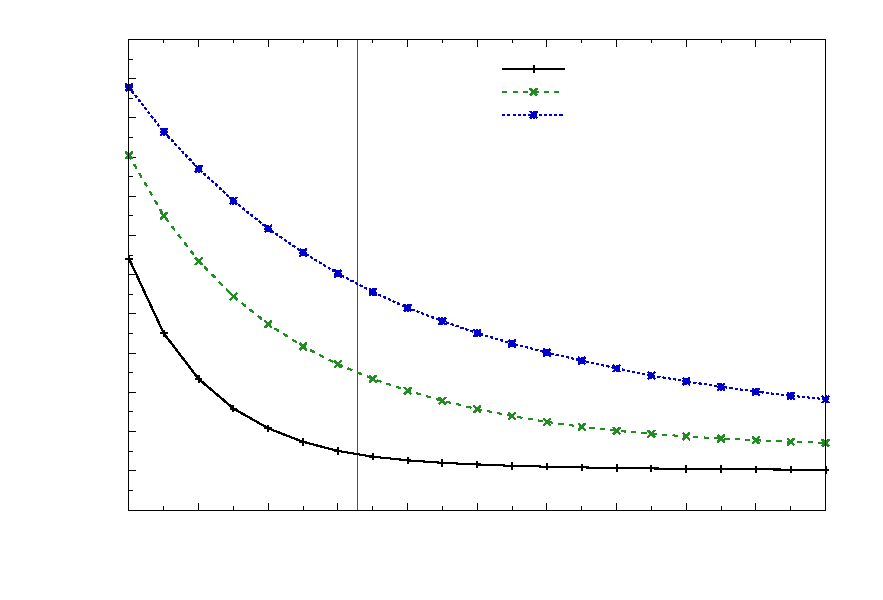
\includegraphics{plot_wind_bess_nmae_hrzn}}%
    \gplfronttext
  \end{picture}%
\endgroup

	}
	\caption[NMAE of wind power dispatch with battery energy storage for control horizons of varying length]{Normalised mean absolute error (NMAE) for the Snowtown wind farm with generation capacity of 1.0~p.u.\ coupled with utility-scale batteries of varying size.  The MPC controller optimises wind power dispatch with battery energy storage over 30-, 60-, and 90-minute prediction/control horizons.  NMAE is calculated as the absolute difference between scheduled power and power dispatched to the grid divided by nameplate generation capacity.} 
	\label{fig:wind_bess_nmae_hrzn}
\end{figure*}

AEMO measures the accuracy of forecasts produced by AWEFS for a range of forecast horizons.  The most common measure of forecast accuracy is normalised mean absolute error (NMAE).  It is calculated as the absolute difference between forecast and actual output divided by nameplate generation capacity.  In order to measure the effect of utility-scale batteries of varying size on firming wind power dispatch, we redefine NMAE to be the absolute difference between scheduled power and power dispatched to the grid divided by nameplate generation capacity.  Observe that in the absence of battery energy storage the two definitions are equivalent.

Figure~\ref{fig:wind_bess_nmae_hrzn} plots NMAE against battery energy capacity for 30-, 60- and 90-minute control horizons.  Unsurprisingly, forecast accuracy improves as the forecast horizon shortens.  Recall that power is scheduled ahead of any given dispatch interval by the length of the control horizon.  With fast start gas turbines capable of reaching full load within 30 minutes, we focus our analysis on virtual trials with a 30-minute control horizon.  For the Snowtown wind farm with a generation capacity of 1.0~p.u.\ and no battery energy storage, NMAE is 6.4\%.  It falls to 1.0\% when a battery with energy capacity of 1.0~p.u.\ is coupled to the wind farm.  But, a much smaller battery will achieve most of this reduction in NMAE.  When a battery with energy capacity of only 0.3~p.u.\ is coupled to the Snowtown wind farm, NMAE drops to 1.5\%.

The proportion of dispatch intervals over the simulation horizon in which power dispatched to the grid is less than scheduled power falls from 54.6\% for no battery energy storage to 24.5\% when a battery with energy capacity of 0.30~p.u.\ is coupled to the Snowtown wind farm (Figure~\ref{fig:wind_bess_nmae_deficit}).  Calculating NMAE only for dispatch intervals in which power dispatched to the grid is less than scheduled power, we find that it lies in a fairly narrow range across battery sizes examined in the virtual trials --- 6.1\% with no battery energy storage, and between 4.5\% and 4.7\% for batteries with energy capacity ranging from 0.3~p.u.\ to 1.0~p.u.  The serial correlation of wind forecast errors means that when the battery falls to its minimum SOC, power dispatched to the grid during the next dispatch interval is likely to be less than scheduled power.  That is, actual wind power is likely to be less than forecast, and the wind farm is, in effect, operating with no battery energy storage.  Figure~\ref{fig:wind_bess_soc} plots SOC of a battery with energy capacity of 0.3~p.u.\ over the simulation horizon.

In an attempt to further reduce NMAE, we conducted virtual trials in which scheduled power is ``curtailed'' on the basis of energy capacity and SOC of the battery.  We consider cases where curtailment is capped at 5\% and 10\% of battery energy capacity.  For dispatch intervals in which battery SOC exceeds 50\%, scheduled power for the $n\textsuperscript{th}$ time interval of the prediction horizon is set to the corresponding 5-minute pre-dispatch UIGF forecast, as is done in the virtual trials reported above.  For dispatch intervals in which battery SOC is less than 50\%, scheduled power is set to the 5-minute pre-dispatch UIGF forecast less an amount between zero and maximum curtailment, which depends linearly on battery SOC (i.e., zero at 50\% SOC and maximum curtailment at minimum SOC).  Figure~\ref{fig:wind_bess_nmae} plots NMAE against battery energy capacity for virtual trials in which scheduled power is curtailed.  Supposing that a utility-scale battery with energy capacity of 0.3~p.u.\ is coupled to the Snowtown wind farm with generation capacity of 1.0~p.u., and assuming a 30-minute control horizon, NMAE is 1.22\% (respectively, 1.10\%) when curtailment is capped at 5\% (10\%) of battery energy capacity.  This compares with an NMAE of 1.51\% with no curtailment of scheduled power.

\begin{figure}[!t]
	\centering
	\scalebox{0.55}{
		% GNUPLOT: LaTeX picture with Postscript
\begingroup
  \makeatletter
  \providecommand\color[2][]{%
    \GenericError{(gnuplot) \space\space\space\@spaces}{%
      Package color not loaded in conjunction with
      terminal option `colourtext'%
    }{See the gnuplot documentation for explanation.%
    }{Either use 'blacktext' in gnuplot or load the package
      color.sty in LaTeX.}%
    \renewcommand\color[2][]{}%
  }%
  \providecommand\includegraphics[2][]{%
    \GenericError{(gnuplot) \space\space\space\@spaces}{%
      Package graphicx or graphics not loaded%
    }{See the gnuplot documentation for explanation.%
    }{The gnuplot epslatex terminal needs graphicx.sty or graphics.sty.}%
    \renewcommand\includegraphics[2][]{}%
  }%
  \providecommand\rotatebox[2]{#2}%
  \@ifundefined{ifGPcolor}{%
    \newif\ifGPcolor
    \GPcolorfalse
  }{}%
  \@ifundefined{ifGPblacktext}{%
    \newif\ifGPblacktext
    \GPblacktexttrue
  }{}%
  % define a \g@addto@macro without @ in the name:
  \let\gplgaddtomacro\g@addto@macro
  % define empty templates for all commands taking text:
  \gdef\gplbacktext{}%
  \gdef\gplfronttext{}%
  \makeatother
  \ifGPblacktext
    % no textcolor at all
    \def\colorrgb#1{}%
    \def\colorgray#1{}%
  \else
    % gray or color?
    \ifGPcolor
      \def\colorrgb#1{\color[rgb]{#1}}%
      \def\colorgray#1{\color[gray]{#1}}%
      \expandafter\def\csname LTw\endcsname{\color{white}}%
      \expandafter\def\csname LTb\endcsname{\color{black}}%
      \expandafter\def\csname LTa\endcsname{\color{black}}%
      \expandafter\def\csname LT0\endcsname{\color[rgb]{1,0,0}}%
      \expandafter\def\csname LT1\endcsname{\color[rgb]{0,1,0}}%
      \expandafter\def\csname LT2\endcsname{\color[rgb]{0,0,1}}%
      \expandafter\def\csname LT3\endcsname{\color[rgb]{1,0,1}}%
      \expandafter\def\csname LT4\endcsname{\color[rgb]{0,1,1}}%
      \expandafter\def\csname LT5\endcsname{\color[rgb]{1,1,0}}%
      \expandafter\def\csname LT6\endcsname{\color[rgb]{0,0,0}}%
      \expandafter\def\csname LT7\endcsname{\color[rgb]{1,0.3,0}}%
      \expandafter\def\csname LT8\endcsname{\color[rgb]{0.5,0.5,0.5}}%
    \else
      % gray
      \def\colorrgb#1{\color{black}}%
      \def\colorgray#1{\color[gray]{#1}}%
      \expandafter\def\csname LTw\endcsname{\color{white}}%
      \expandafter\def\csname LTb\endcsname{\color{black}}%
      \expandafter\def\csname LTa\endcsname{\color{black}}%
      \expandafter\def\csname LT0\endcsname{\color{black}}%
      \expandafter\def\csname LT1\endcsname{\color{black}}%
      \expandafter\def\csname LT2\endcsname{\color{black}}%
      \expandafter\def\csname LT3\endcsname{\color{black}}%
      \expandafter\def\csname LT4\endcsname{\color{black}}%
      \expandafter\def\csname LT5\endcsname{\color{black}}%
      \expandafter\def\csname LT6\endcsname{\color{black}}%
      \expandafter\def\csname LT7\endcsname{\color{black}}%
      \expandafter\def\csname LT8\endcsname{\color{black}}%
    \fi
  \fi
    \setlength{\unitlength}{0.0500bp}%
    \ifx\gptboxheight\undefined%
      \newlength{\gptboxheight}%
      \newlength{\gptboxwidth}%
      \newsavebox{\gptboxtext}%
    \fi%
    \setlength{\fboxrule}{0.5pt}%
    \setlength{\fboxsep}{1pt}%
\begin{picture}(8162.00,5442.00)%
    \gplgaddtomacro\gplbacktext{%
      \csname LTb\endcsname%%
      \put(946,704){\makebox(0,0)[r]{\strut{}0.0}}%
      \put(946,1080){\makebox(0,0)[r]{\strut{}5.0}}%
      \put(946,1457){\makebox(0,0)[r]{\strut{}10.0}}%
      \put(946,1833){\makebox(0,0)[r]{\strut{}15.0}}%
      \put(946,2210){\makebox(0,0)[r]{\strut{}20.0}}%
      \put(946,2586){\makebox(0,0)[r]{\strut{}25.0}}%
      \put(946,2963){\makebox(0,0)[r]{\strut{}30.0}}%
      \put(946,3339){\makebox(0,0)[r]{\strut{}35.0}}%
      \put(946,3715){\makebox(0,0)[r]{\strut{}40.0}}%
      \put(946,4092){\makebox(0,0)[r]{\strut{}45.0}}%
      \put(946,4468){\makebox(0,0)[r]{\strut{}50.0}}%
      \put(946,4845){\makebox(0,0)[r]{\strut{}55.0}}%
      \put(946,5221){\makebox(0,0)[r]{\strut{}60.0}}%
      \put(1078,484){\makebox(0,0){\strut{}0.00}}%
      \put(1646,484){\makebox(0,0){\strut{}0.10}}%
      \put(2213,484){\makebox(0,0){\strut{}0.20}}%
      \put(2781,484){\makebox(0,0){\strut{}0.30}}%
      \put(3348,484){\makebox(0,0){\strut{}0.40}}%
      \put(3916,484){\makebox(0,0){\strut{}0.50}}%
      \put(4483,484){\makebox(0,0){\strut{}0.60}}%
      \put(5051,484){\makebox(0,0){\strut{}0.70}}%
      \put(5618,484){\makebox(0,0){\strut{}0.80}}%
      \put(6185,484){\makebox(0,0){\strut{}0.90}}%
      \put(6753,484){\makebox(0,0){\strut{}1.00}}%
      \put(6885,704){\makebox(0,0)[l]{\strut{}0.0}}%
      \put(6885,1156){\makebox(0,0)[l]{\strut{}2.0}}%
      \put(6885,1607){\makebox(0,0)[l]{\strut{}4.0}}%
      \put(6885,2059){\makebox(0,0)[l]{\strut{}6.0}}%
      \put(6885,2511){\makebox(0,0)[l]{\strut{}8.0}}%
      \put(6885,2963){\makebox(0,0)[l]{\strut{}10.0}}%
      \put(6885,3414){\makebox(0,0)[l]{\strut{}12.0}}%
      \put(6885,3866){\makebox(0,0)[l]{\strut{}14.0}}%
      \put(6885,4318){\makebox(0,0)[l]{\strut{}16.0}}%
      \put(6885,4769){\makebox(0,0)[l]{\strut{}18.0}}%
      \put(6885,5221){\makebox(0,0)[l]{\strut{}20.0}}%
    }%
    \gplgaddtomacro\gplfronttext{%
      \csname LTb\endcsname%%
      \put(198,2962){\rotatebox{-270}{\makebox(0,0){\strut{}\shortstack{Proportion of dispatch intervals in which\\power dispatched is less than scheduled, \%}}}}%
      \put(7809,2962){\rotatebox{-270}{\makebox(0,0){\strut{}\shortstack{Normalised mean absolute error for dispatch intervals\\in which power dispatched is less than scheduled, \%}}}}%
      \put(3915,154){\makebox(0,0){\strut{}Battery power rating/ energy capacity, p.u.}}%
    }%
    \gplbacktext
    \put(0,0){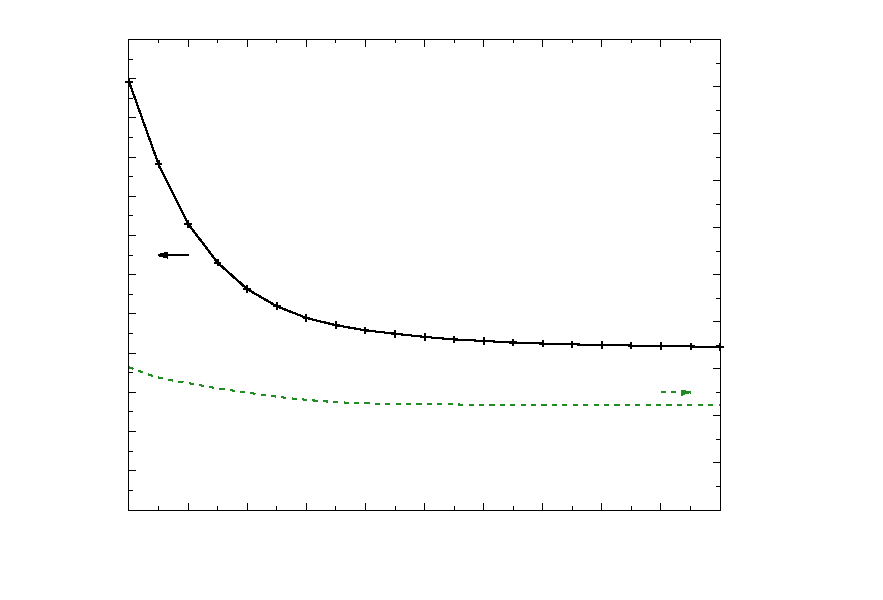
\includegraphics{plot_wind_bess_nmae_deficit}}%
    \gplfronttext
  \end{picture}%
\endgroup

	}
	\caption[Proportion of dispatch intervals in which power dispatched to the grid is less than scheduled power]{Proportion of dispatch intervals and NMAE for dispatch intervals in which power dispatch to the grid is less than scheduled power, supposing that the Snowtown wind farm with generation capacity of 1.0~p.u.\ is coupled with utility-scale batteries of varying size.} 
	\label{fig:wind_bess_nmae_deficit}
\end{figure}

\begin{figure}[!b]
	\centering
	\scalebox{0.55}{
		% GNUPLOT: LaTeX picture with Postscript
\begingroup
  \makeatletter
  \providecommand\color[2][]{%
    \GenericError{(gnuplot) \space\space\space\@spaces}{%
      Package color not loaded in conjunction with
      terminal option `colourtext'%
    }{See the gnuplot documentation for explanation.%
    }{Either use 'blacktext' in gnuplot or load the package
      color.sty in LaTeX.}%
    \renewcommand\color[2][]{}%
  }%
  \providecommand\includegraphics[2][]{%
    \GenericError{(gnuplot) \space\space\space\@spaces}{%
      Package graphicx or graphics not loaded%
    }{See the gnuplot documentation for explanation.%
    }{The gnuplot epslatex terminal needs graphicx.sty or graphics.sty.}%
    \renewcommand\includegraphics[2][]{}%
  }%
  \providecommand\rotatebox[2]{#2}%
  \@ifundefined{ifGPcolor}{%
    \newif\ifGPcolor
    \GPcolorfalse
  }{}%
  \@ifundefined{ifGPblacktext}{%
    \newif\ifGPblacktext
    \GPblacktexttrue
  }{}%
  % define a \g@addto@macro without @ in the name:
  \let\gplgaddtomacro\g@addto@macro
  % define empty templates for all commands taking text:
  \gdef\gplbacktext{}%
  \gdef\gplfronttext{}%
  \makeatother
  \ifGPblacktext
    % no textcolor at all
    \def\colorrgb#1{}%
    \def\colorgray#1{}%
  \else
    % gray or color?
    \ifGPcolor
      \def\colorrgb#1{\color[rgb]{#1}}%
      \def\colorgray#1{\color[gray]{#1}}%
      \expandafter\def\csname LTw\endcsname{\color{white}}%
      \expandafter\def\csname LTb\endcsname{\color{black}}%
      \expandafter\def\csname LTa\endcsname{\color{black}}%
      \expandafter\def\csname LT0\endcsname{\color[rgb]{1,0,0}}%
      \expandafter\def\csname LT1\endcsname{\color[rgb]{0,1,0}}%
      \expandafter\def\csname LT2\endcsname{\color[rgb]{0,0,1}}%
      \expandafter\def\csname LT3\endcsname{\color[rgb]{1,0,1}}%
      \expandafter\def\csname LT4\endcsname{\color[rgb]{0,1,1}}%
      \expandafter\def\csname LT5\endcsname{\color[rgb]{1,1,0}}%
      \expandafter\def\csname LT6\endcsname{\color[rgb]{0,0,0}}%
      \expandafter\def\csname LT7\endcsname{\color[rgb]{1,0.3,0}}%
      \expandafter\def\csname LT8\endcsname{\color[rgb]{0.5,0.5,0.5}}%
    \else
      % gray
      \def\colorrgb#1{\color{black}}%
      \def\colorgray#1{\color[gray]{#1}}%
      \expandafter\def\csname LTw\endcsname{\color{white}}%
      \expandafter\def\csname LTb\endcsname{\color{black}}%
      \expandafter\def\csname LTa\endcsname{\color{black}}%
      \expandafter\def\csname LT0\endcsname{\color{black}}%
      \expandafter\def\csname LT1\endcsname{\color{black}}%
      \expandafter\def\csname LT2\endcsname{\color{black}}%
      \expandafter\def\csname LT3\endcsname{\color{black}}%
      \expandafter\def\csname LT4\endcsname{\color{black}}%
      \expandafter\def\csname LT5\endcsname{\color{black}}%
      \expandafter\def\csname LT6\endcsname{\color{black}}%
      \expandafter\def\csname LT7\endcsname{\color{black}}%
      \expandafter\def\csname LT8\endcsname{\color{black}}%
    \fi
  \fi
    \setlength{\unitlength}{0.0500bp}%
    \ifx\gptboxheight\undefined%
      \newlength{\gptboxheight}%
      \newlength{\gptboxwidth}%
      \newsavebox{\gptboxtext}%
    \fi%
    \setlength{\fboxrule}{0.5pt}%
    \setlength{\fboxsep}{1pt}%
\begin{picture}(8162.00,5442.00)%
    \gplgaddtomacro\gplbacktext{%
      \csname LTb\endcsname%%
      \put(946,440){\makebox(0,0)[r]{\strut{}0.0}}%
      \put(946,918){\makebox(0,0)[r]{\strut{}3.0}}%
      \put(946,1396){\makebox(0,0)[r]{\strut{}5.9}}%
      \put(946,1874){\makebox(0,0)[r]{\strut{}8.9}}%
      \put(946,2352){\makebox(0,0)[r]{\strut{}11.9}}%
      \put(946,2831){\makebox(0,0)[r]{\strut{}14.9}}%
      \put(946,3309){\makebox(0,0)[r]{\strut{}17.8}}%
      \put(946,3787){\makebox(0,0)[r]{\strut{}20.8}}%
      \put(946,4265){\makebox(0,0)[r]{\strut{}23.8}}%
      \put(946,4743){\makebox(0,0)[r]{\strut{}26.7}}%
      \put(946,5221){\makebox(0,0)[r]{\strut{}29.7}}%
      \put(1141,-275){\rotatebox{90}{\makebox(0,0)[l]{\strut{}Apr-17}}}%
      \put(1608,-275){\rotatebox{90}{\makebox(0,0)[l]{\strut{}May-17}}}%
      \put(2090,-275){\rotatebox{90}{\makebox(0,0)[l]{\strut{}Jun-17}}}%
      \put(2557,-275){\rotatebox{90}{\makebox(0,0)[l]{\strut{}Jul-17}}}%
      \put(3040,-275){\rotatebox{90}{\makebox(0,0)[l]{\strut{}Aug-17}}}%
      \put(3522,-275){\rotatebox{90}{\makebox(0,0)[l]{\strut{}Sep-17}}}%
      \put(3989,-275){\rotatebox{90}{\makebox(0,0)[l]{\strut{}Oct-17}}}%
      \put(4472,-275){\rotatebox{90}{\makebox(0,0)[l]{\strut{}Nov-17}}}%
      \put(4939,-275){\rotatebox{90}{\makebox(0,0)[l]{\strut{}Dec-17}}}%
      \put(5421,-275){\rotatebox{90}{\makebox(0,0)[l]{\strut{}Jan-18}}}%
      \put(5904,-275){\rotatebox{90}{\makebox(0,0)[l]{\strut{}Feb-18}}}%
      \put(6340,-275){\rotatebox{90}{\makebox(0,0)[l]{\strut{}Mar-18}}}%
      \put(6822,-275){\rotatebox{90}{\makebox(0,0)[l]{\strut{}Apr-18}}}%
      \put(7017,440){\makebox(0,0)[l]{\strut{}0}}%
      \put(7017,918){\makebox(0,0)[l]{\strut{}10}}%
      \put(7017,1396){\makebox(0,0)[l]{\strut{}20}}%
      \put(7017,1874){\makebox(0,0)[l]{\strut{}30}}%
      \put(7017,2352){\makebox(0,0)[l]{\strut{}40}}%
      \put(7017,2831){\makebox(0,0)[l]{\strut{}50}}%
      \put(7017,3309){\makebox(0,0)[l]{\strut{}60}}%
      \put(7017,3787){\makebox(0,0)[l]{\strut{}70}}%
      \put(7017,4265){\makebox(0,0)[l]{\strut{}80}}%
      \put(7017,4743){\makebox(0,0)[l]{\strut{}90}}%
      \put(7017,5221){\makebox(0,0)[l]{\strut{}100}}%
    }%
    \gplgaddtomacro\gplfronttext{%
      \csname LTb\endcsname%%
      \put(198,2830){\rotatebox{-270}{\makebox(0,0){\strut{}Battery state of charge, MWh}}}%
      \put(7809,2830){\rotatebox{-270}{\makebox(0,0){\strut{}Battery state of charge, \%}}}%
    }%
    \gplbacktext
    \put(0,0){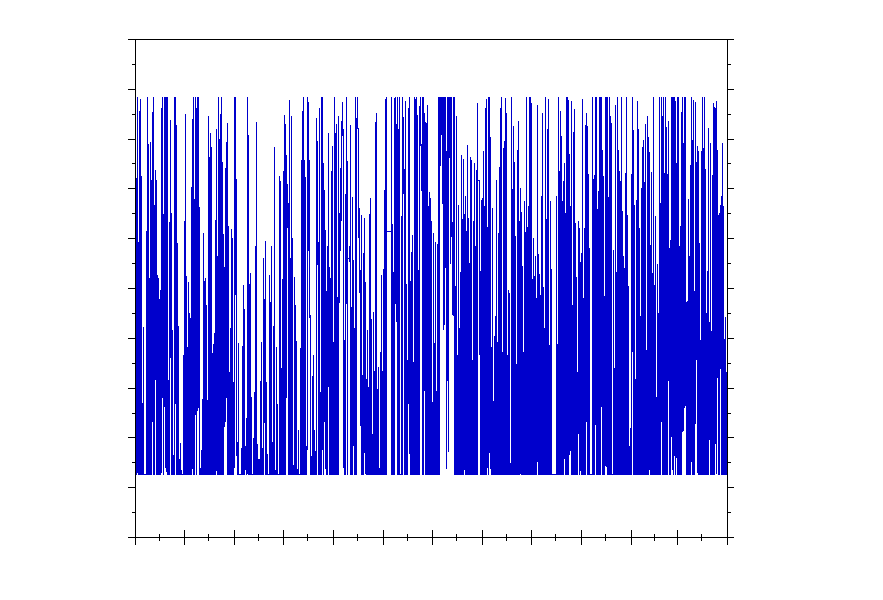
\includegraphics{plot_wind_bess_soc}}%
    \gplfronttext
  \end{picture}%
\endgroup

	}
	\caption[State of charge of the battery over the simulation horizon]{State of charge of a battery with energy capacity of 0.3~p.u.\ coupled to the Snowtown wind farm with generation capacity of 1.0~p.u.\ over the simulation horizon from 1 April 2017 to 31 March 2018.} 
	\label{fig:wind_bess_soc}
\end{figure}

\begin{figure*}[!t]
	\centering
	\scalebox{1.0}{
		% GNUPLOT: LaTeX picture with Postscript
\begingroup
  \makeatletter
  \providecommand\color[2][]{%
    \GenericError{(gnuplot) \space\space\space\@spaces}{%
      Package color not loaded in conjunction with
      terminal option `colourtext'%
    }{See the gnuplot documentation for explanation.%
    }{Either use 'blacktext' in gnuplot or load the package
      color.sty in LaTeX.}%
    \renewcommand\color[2][]{}%
  }%
  \providecommand\includegraphics[2][]{%
    \GenericError{(gnuplot) \space\space\space\@spaces}{%
      Package graphicx or graphics not loaded%
    }{See the gnuplot documentation for explanation.%
    }{The gnuplot epslatex terminal needs graphicx.sty or graphics.sty.}%
    \renewcommand\includegraphics[2][]{}%
  }%
  \providecommand\rotatebox[2]{#2}%
  \@ifundefined{ifGPcolor}{%
    \newif\ifGPcolor
    \GPcolorfalse
  }{}%
  \@ifundefined{ifGPblacktext}{%
    \newif\ifGPblacktext
    \GPblacktexttrue
  }{}%
  % define a \g@addto@macro without @ in the name:
  \let\gplgaddtomacro\g@addto@macro
  % define empty templates for all commands taking text:
  \gdef\gplbacktext{}%
  \gdef\gplfronttext{}%
  \makeatother
  \ifGPblacktext
    % no textcolor at all
    \def\colorrgb#1{}%
    \def\colorgray#1{}%
  \else
    % gray or color?
    \ifGPcolor
      \def\colorrgb#1{\color[rgb]{#1}}%
      \def\colorgray#1{\color[gray]{#1}}%
      \expandafter\def\csname LTw\endcsname{\color{white}}%
      \expandafter\def\csname LTb\endcsname{\color{black}}%
      \expandafter\def\csname LTa\endcsname{\color{black}}%
      \expandafter\def\csname LT0\endcsname{\color[rgb]{1,0,0}}%
      \expandafter\def\csname LT1\endcsname{\color[rgb]{0,1,0}}%
      \expandafter\def\csname LT2\endcsname{\color[rgb]{0,0,1}}%
      \expandafter\def\csname LT3\endcsname{\color[rgb]{1,0,1}}%
      \expandafter\def\csname LT4\endcsname{\color[rgb]{0,1,1}}%
      \expandafter\def\csname LT5\endcsname{\color[rgb]{1,1,0}}%
      \expandafter\def\csname LT6\endcsname{\color[rgb]{0,0,0}}%
      \expandafter\def\csname LT7\endcsname{\color[rgb]{1,0.3,0}}%
      \expandafter\def\csname LT8\endcsname{\color[rgb]{0.5,0.5,0.5}}%
    \else
      % gray
      \def\colorrgb#1{\color{black}}%
      \def\colorgray#1{\color[gray]{#1}}%
      \expandafter\def\csname LTw\endcsname{\color{white}}%
      \expandafter\def\csname LTb\endcsname{\color{black}}%
      \expandafter\def\csname LTa\endcsname{\color{black}}%
      \expandafter\def\csname LT0\endcsname{\color{black}}%
      \expandafter\def\csname LT1\endcsname{\color{black}}%
      \expandafter\def\csname LT2\endcsname{\color{black}}%
      \expandafter\def\csname LT3\endcsname{\color{black}}%
      \expandafter\def\csname LT4\endcsname{\color{black}}%
      \expandafter\def\csname LT5\endcsname{\color{black}}%
      \expandafter\def\csname LT6\endcsname{\color{black}}%
      \expandafter\def\csname LT7\endcsname{\color{black}}%
      \expandafter\def\csname LT8\endcsname{\color{black}}%
    \fi
  \fi
    \setlength{\unitlength}{0.0500bp}%
    \ifx\gptboxheight\undefined%
      \newlength{\gptboxheight}%
      \newlength{\gptboxwidth}%
      \newsavebox{\gptboxtext}%
    \fi%
    \setlength{\fboxrule}{0.5pt}%
    \setlength{\fboxsep}{1pt}%
\begin{picture}(8162.00,5442.00)%
    \gplgaddtomacro\gplbacktext{%
      \csname LTb\endcsname%%
      \put(814,704){\makebox(0,0)[r]{\strut{}0.0}}%
      \put(814,1269){\makebox(0,0)[r]{\strut{}1.0}}%
      \put(814,1833){\makebox(0,0)[r]{\strut{}2.0}}%
      \put(814,2398){\makebox(0,0)[r]{\strut{}3.0}}%
      \put(814,2963){\makebox(0,0)[r]{\strut{}4.0}}%
      \put(814,3527){\makebox(0,0)[r]{\strut{}5.0}}%
      \put(814,4092){\makebox(0,0)[r]{\strut{}6.0}}%
      \put(814,4656){\makebox(0,0)[r]{\strut{}7.0}}%
      \put(814,5221){\makebox(0,0)[r]{\strut{}8.0}}%
      \put(946,484){\makebox(0,0){\strut{}0.00}}%
      \put(1628,484){\makebox(0,0){\strut{}0.10}}%
      \put(2310,484){\makebox(0,0){\strut{}0.20}}%
      \put(2992,484){\makebox(0,0){\strut{}0.30}}%
      \put(3674,484){\makebox(0,0){\strut{}0.40}}%
      \put(4356,484){\makebox(0,0){\strut{}0.50}}%
      \put(5037,484){\makebox(0,0){\strut{}0.60}}%
      \put(5719,484){\makebox(0,0){\strut{}0.70}}%
      \put(6401,484){\makebox(0,0){\strut{}0.80}}%
      \put(7083,484){\makebox(0,0){\strut{}0.90}}%
      \put(7765,484){\makebox(0,0){\strut{}1.00}}%
      \put(3401,2963){\makebox(0,0)[l]{\strut{}\small Capacity factor = 0.349}}%
    }%
    \gplgaddtomacro\gplfronttext{%
      \csname LTb\endcsname%%
      \put(198,2962){\rotatebox{-270}{\makebox(0,0){\strut{}Normalised mean absolute error, \%}}}%
      \put(4355,154){\makebox(0,0){\strut{}Battery power rating/ energy capacity, p.u.}}%
      \csname LTb\endcsname%%
      \put(5521,5048){\makebox(0,0)[l]{\strut{}\small No curtailment}}%
      \csname LTb\endcsname%%
      \put(5521,4828){\makebox(0,0)[l]{\strut{}\small Maximum curtailment 5\%}}%
      \csname LTb\endcsname%%
      \put(5521,4608){\makebox(0,0)[l]{\strut{}\small Maximum curtailment 10\%}}%
    }%
    \gplbacktext
    \put(0,0){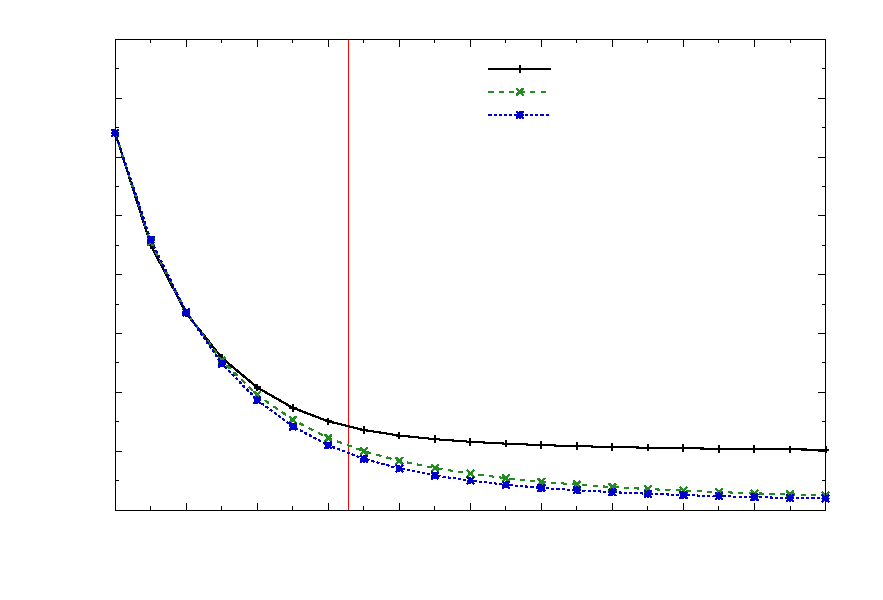
\includegraphics{plot_wind_bess_nmae}}%
    \gplfronttext
  \end{picture}%
\endgroup

	}
	\caption[NMAE of wind power dispatch with battery energy storage when scheduled power is curtailed]{Normalised mean absolute error for the Snowtown wind farm with generation capacity of 1.0~p.u.\ coupled with utility-scale batteries of varying size.  Scheduled power is curtailed on the basis of energy capacity and state of charge of the battery.} 
	\label{fig:wind_bess_nmae}
\end{figure*}

Relative to wind power dispatch with no energy storage, there is a loss of energy attributable to charge/discharge efficiency of the battery coupled to the wind farm (i.e., losses due to the transformation of electrical energy to chemical energy and then back to electrical energy).  In the case of a battery with energy capacity of 0.3~p.u.\ and charge/discharge efficiency of 80\% coupled to the Snowtown wind farm, we calculate the energy loss as 1.41\% of energy dispatched to the grid.  Curtailing scheduled power increases the amount of energy supplied to and discharged from the battery over the simulation horizon, and hence energy losses.  Though, with curtailment of scheduled power capped at 10\% of battery energy capacity (0.3~p.u.), the additional energy loss relative to no curtailment is about one-tenth of one per cent of energy dispatched to the grid.

%%=========================================================================================%%
%% CONCLUSION																				%%
%%=========================================================================================%%
\section{Conclusion}\label{sect:conclusion}
In this paper we develop a multi-period incremental state-space model of wind power dispatch with battery energy storage.  It improves on prior models in the literature by properly accounting for battery charge/discharge efficiency and penalising control effort.  We apply MPC with mixed integer quadratic programming to minimise the tracking error of power (wind and battery) dispatched to the grid relative to power scheduled during pre-dispatch according to UIGF forecasts.  Supposing that a utility-scale battery with energy capacity of 0.3~p.u.\ is coupled to the Snowtown wind farm with generation capacity of 1.0~p.u., NMAE of power dispatched to the grid relative to scheduled power is 1.5\% compared with 6.4\% with no battery energy storage.  We conjecture that firming wind power dispatch with battery energy storage would dampen the volatility of wholesales electricity prices, leading to lower prices.

With around 1,600 MW of existing wind generation capacity and 3,200 MW of committed or proposed wind generation capacity in SA \cite{SAER17}, coupling utility-scale batteries to wind farms would serve to address key recommendations in the Finkel Report \cite{FINKEL17}.  Specifically, requiring ``new generators to have fast frequency response capability'', and including in the Generator Reliability Obligation ``a forward looking regional reliability assessment, taking into account emerging system needs, to inform requirements on new generators to ensure adequate dispatchable capacity is present in the region.''  Moreover, AEMO, in its National Transmission Network Development Plan \cite{NTNDP16}, recommends ``scheduled battery storage'' as a solution for providing frequency regulation to bolster resilience of the SA power system.  Along the lines of these recommendations, future research could examine the efficacy of provisioning frequency regulation from wind farms coupled with utility-scale batteries, and market designs that would fairly compensate generator for providing ancillary services in regions with a high penetration of variable renewable energy resources.

%%=========================================================================================%%
%% ACKNOWLEDGEMENTS																		%%
%%=========================================================================================%%
\section*{Acknowledgments}
We acknowledge the support of Tilt Renewables, who have granted the University of Adelaide access to their confidential unconstrained intermittent generation forecasts for the Snowtown wind farm.  Funding for this research is provided by the Australian Research Council through Grant \textit{CE140100049}.

%%=========================================================================================%%
%% REFERENCES																				%%
%%=========================================================================================%%
\bibliography{sagridnat}

\end{document}